\documentclass[../main.tex]{subfiles}

\begin{document}

\section{Results} \label{sec:results}

To test the code, we decided to run it with \textit{1}, \textit{2}, \textit{4} and \textit{8} threads, we could remove the \textit{1} and \textit{8} thread execution, since they will be worse than the serial and the \textit{4} thread execution, respectively, since our machines only have 4 cores.

To calculate the speedup and efficiency we used the following formulas:

\begin{equation}
    \begin{split}
        S&=\frac{T_1}{T_n}
    \end{split}
\end{equation}

\begin{equation}
    \begin{split}
        E&=\frac{S}{n}=\frac{T_1}{n * T_n}
    \end{split}
\end{equation}

\textbf{IMPORTANT:} For the calculation of efficiency, as we are evaluating the threading scalability, we will use as \textit{n} the number of used threads instead of the ones that the machine has. This means that in the execution of \textit{8} threads, we will use \textit{8} instead of \textit{4}.

\subsection{\textit{100 steps} results}

First, we will show the executions using \textit{100 steps} in \textit{Figure \ref{fig:100-steps}}, \textit{Figure \ref{fig:100-steps-speedup}} and \textit{Figure \ref{fig:100-steps-efficiency}}. Notice the logarithmic Y-axis in the time graph and that the speedup and efficiency graph contains a column for `Theoretical speedup' which is [1, 4] since the machine we will run the code on has 4 cores.


\begin{figure}[!htb]
    \centering
    \label{fig:100-steps-all}
    \begin{subfigure}{0.7\textwidth}
        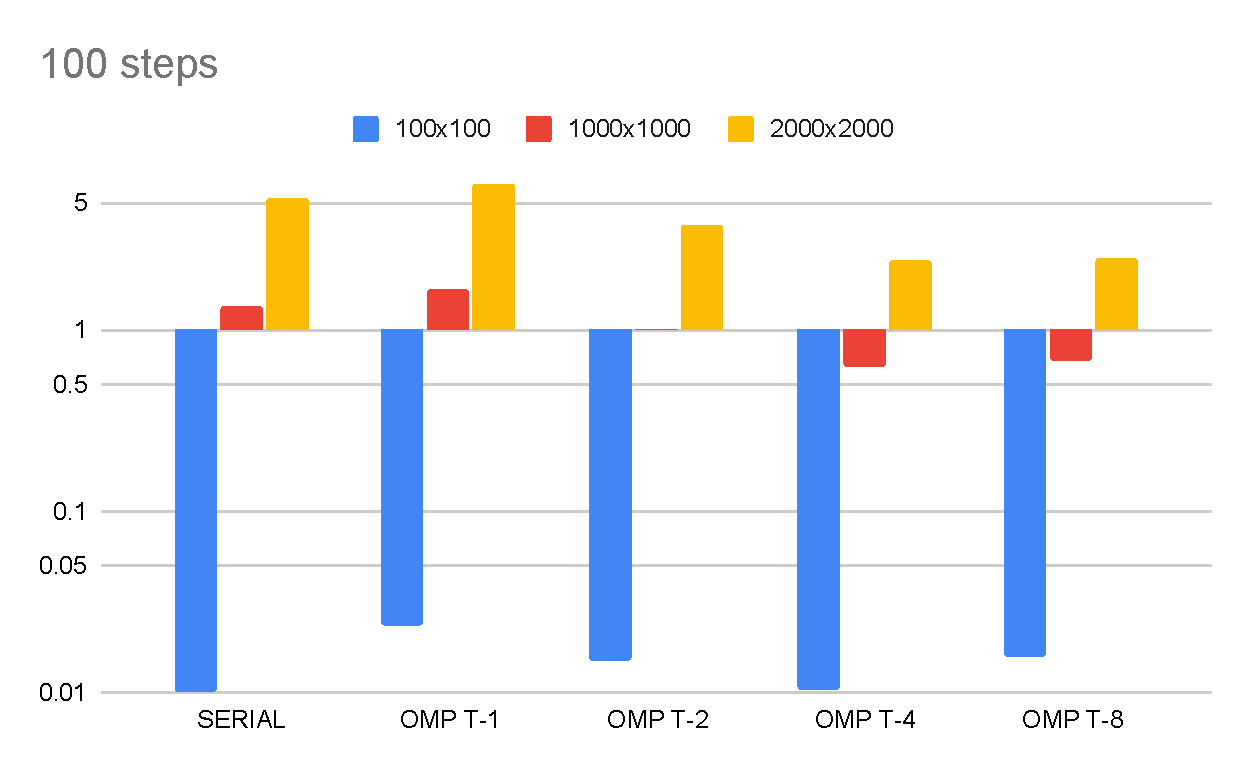
\includegraphics[width=0.9\linewidth]{  \subfix{../media/figures/100 steps.pdf}}
        \caption{Execution time comparison between different matrix sizes}
        \label{fig:100-steps}
    \end{subfigure}
    \begin{subfigure}{0.7\textwidth}
        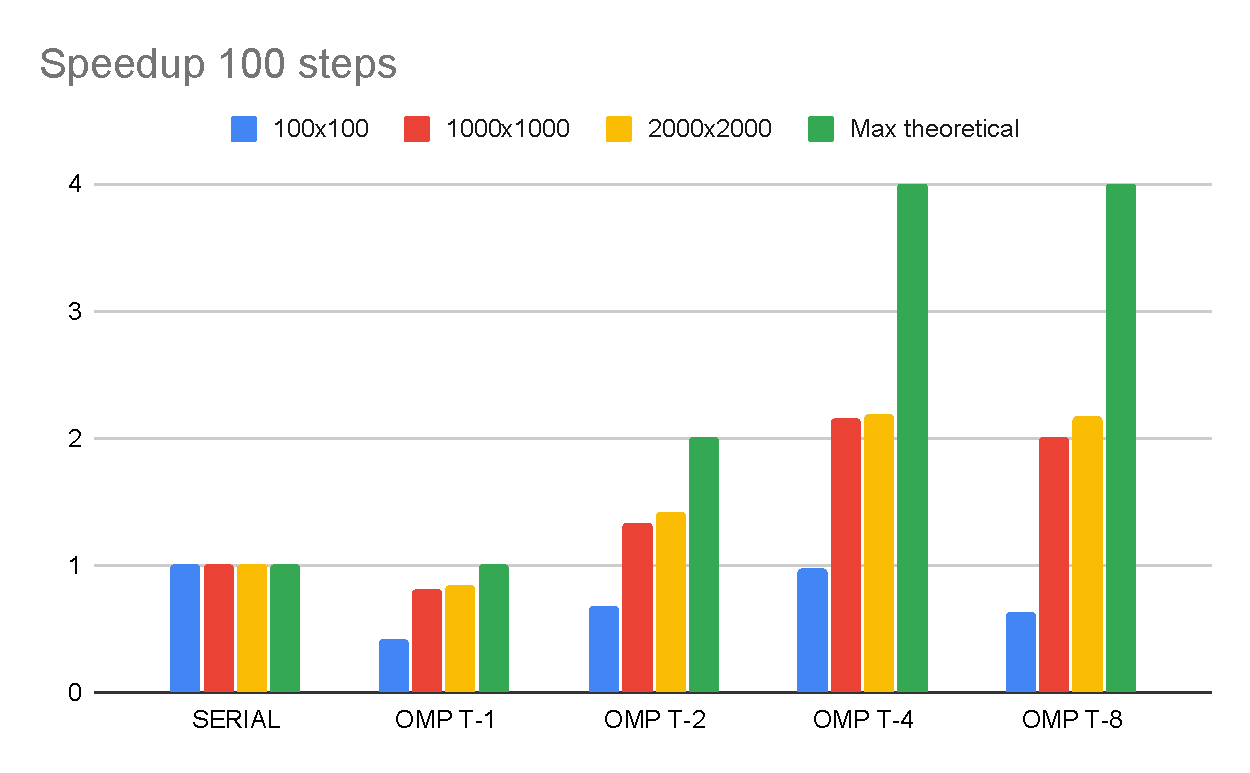
\includegraphics[width=0.9\linewidth]{\subfix{../media/figures/Speedup 100 steps.pdf}}
        \caption{Speedup comparison of the different executions}
        \label{fig:100-steps-speedup}
    \end{subfigure}
    \begin{subfigure}{0.7\textwidth}
        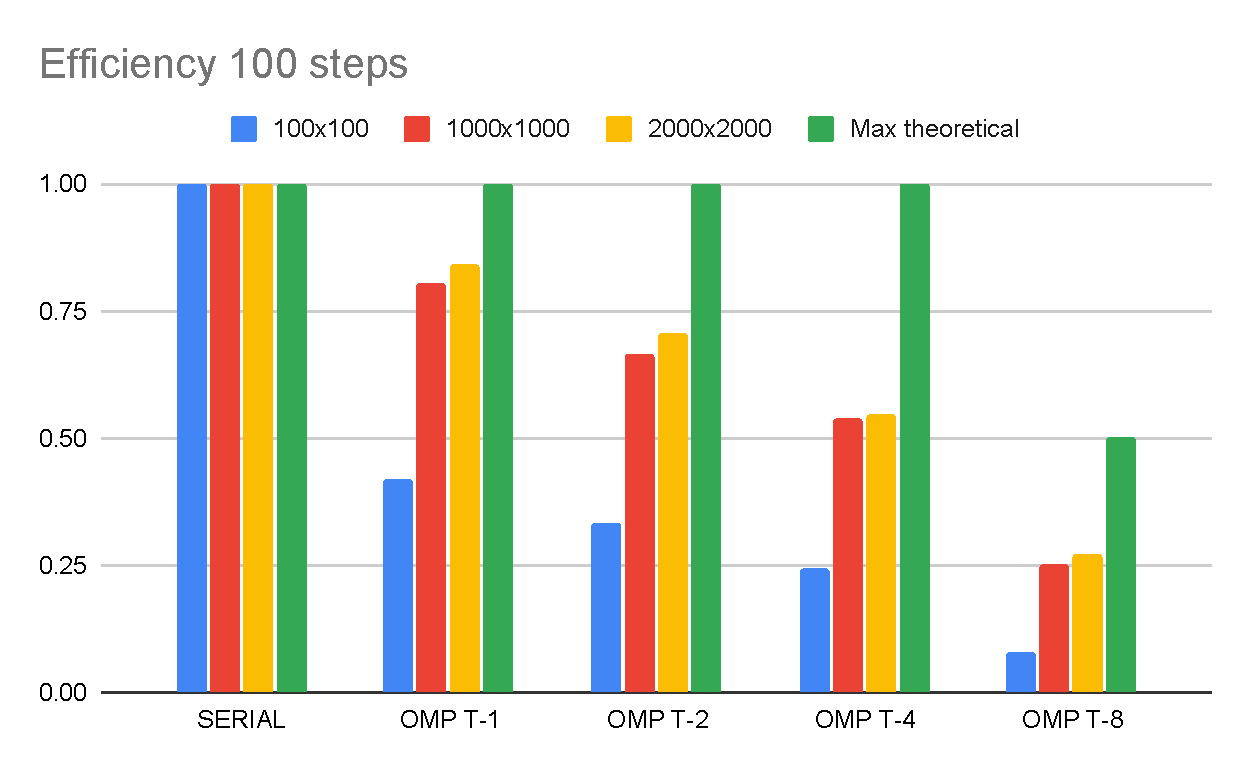
\includegraphics[width=0.9\linewidth]{\subfix{../media/figures/Efficiency 100 steps.pdf}}
        \caption{Efficiency comparison of the different executions}
        \label{fig:100-steps-efficiency}
    \end{subfigure}
    \caption{Time, speedup and efficiency graphs of \textit{100 steps} execution}
\end{figure}

\subsection{\textit{1000 steps} results}

Executions using \textit{1000 steps}, \textit{Figure \ref{fig:1000-steps}}, \textit{Figure \ref{fig:1000-steps-speedup}} and \textit{Figure \ref{fig:1000-steps-efficiency}}. 


\begin{figure}[!htb]
    \centering
    \label{fig:1000-steps-all}
    \begin{subfigure}{0.7\textwidth}
        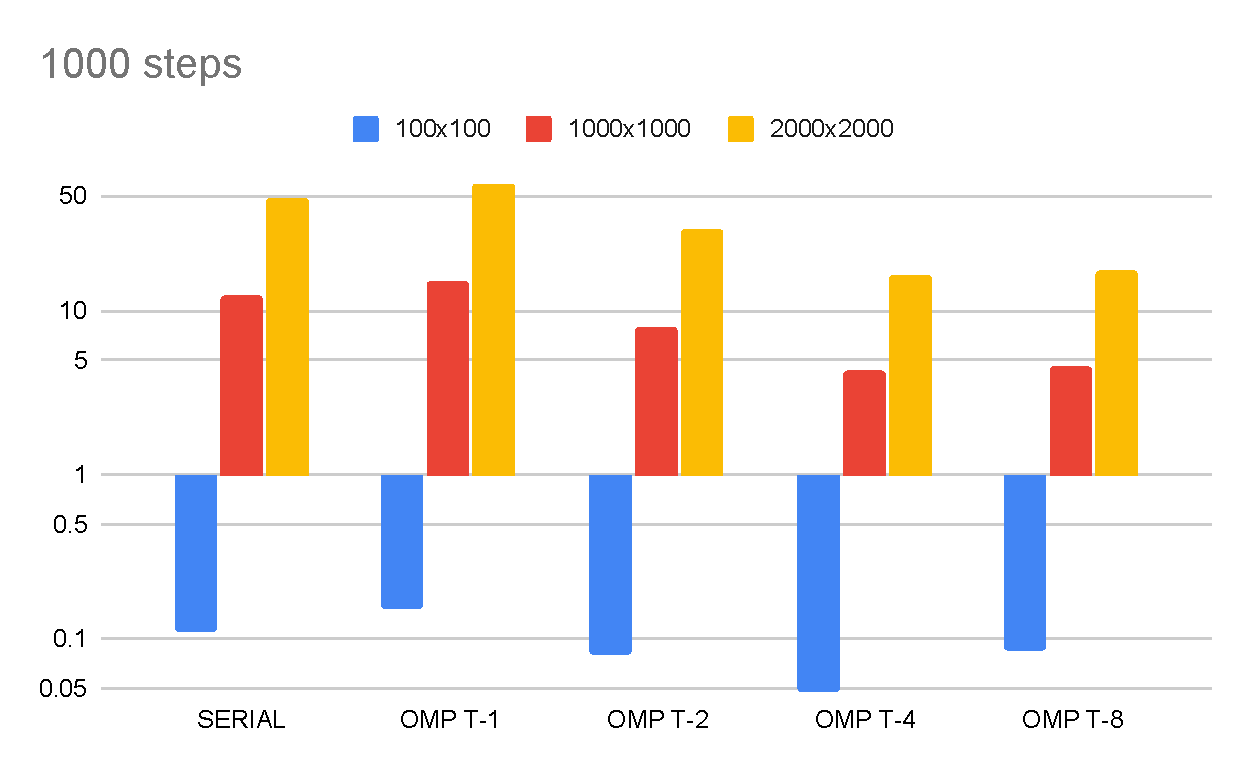
\includegraphics[width=0.9\linewidth]{\subfix{../media/figures/1000 steps.pdf}}
        \caption{Execution time comparison between different matrix sizes}
        \label{fig:1000-steps}
    \end{subfigure}
    \begin{subfigure}{0.7\textwidth}
        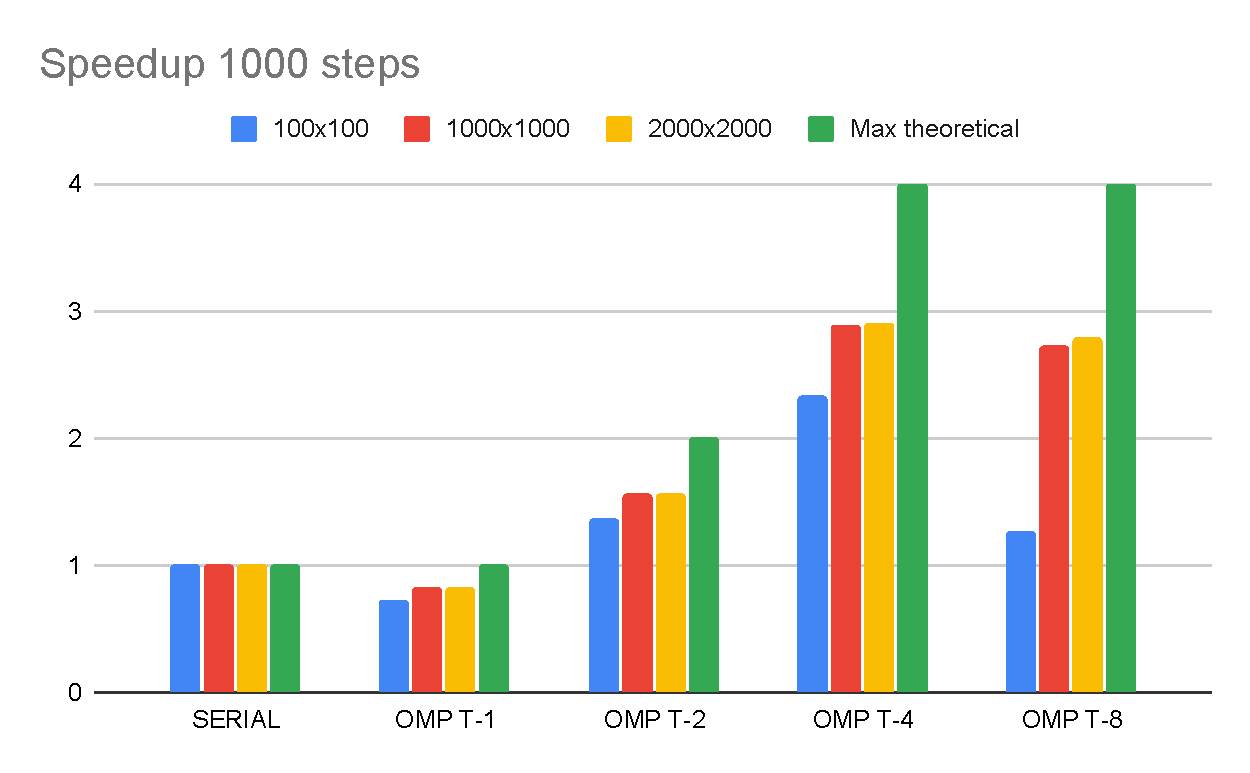
\includegraphics[width=0.9\linewidth]{\subfix{../media/figures/Speedup 1000 steps.pdf}}
        \caption{Speedup comparison of the different executions}
        \label{fig:1000-steps-speedup}
    \end{subfigure}
    \begin{subfigure}{0.7\textwidth}
        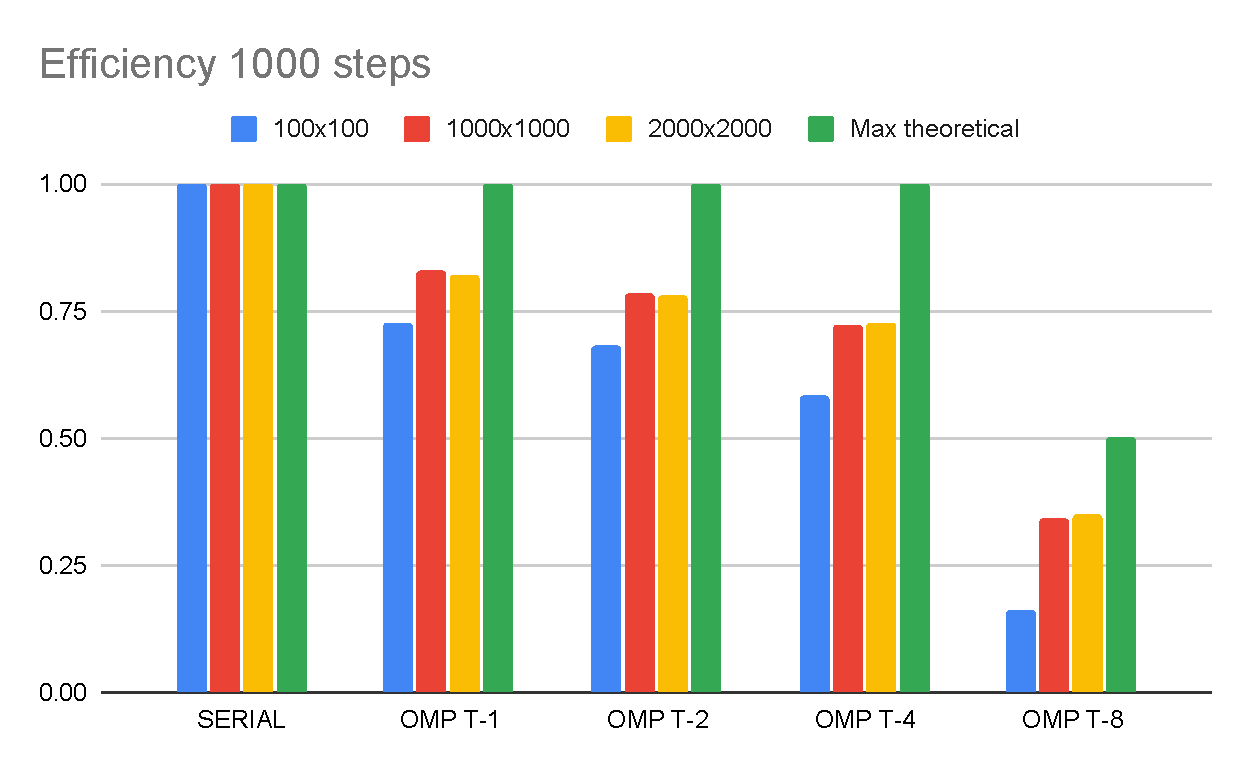
\includegraphics[width=0.9\linewidth]{\subfix{../media/figures/Efficiency 1000 steps.pdf}}
        \caption{Efficiency comparison of the different executions}
        \label{fig:1000-steps-efficiency}
    \end{subfigure}
    \caption{Time, speedup and efficiency graphs of \textit{1000 steps} execution}
\end{figure}

\subsection{\textit{10000 steps} results}

Executions using \textit{10000 steps}, \textit{Figure \ref{fig:10000-steps}}, \textit{Figure \ref{fig:10000-steps-speedup}} and \textit{Figure \ref{fig:10000-steps-efficiency}}. 


\begin{figure}[!htb]
    \centering
    \label{fig:10000-steps-all}
    \begin{subfigure}{0.7\textwidth}
        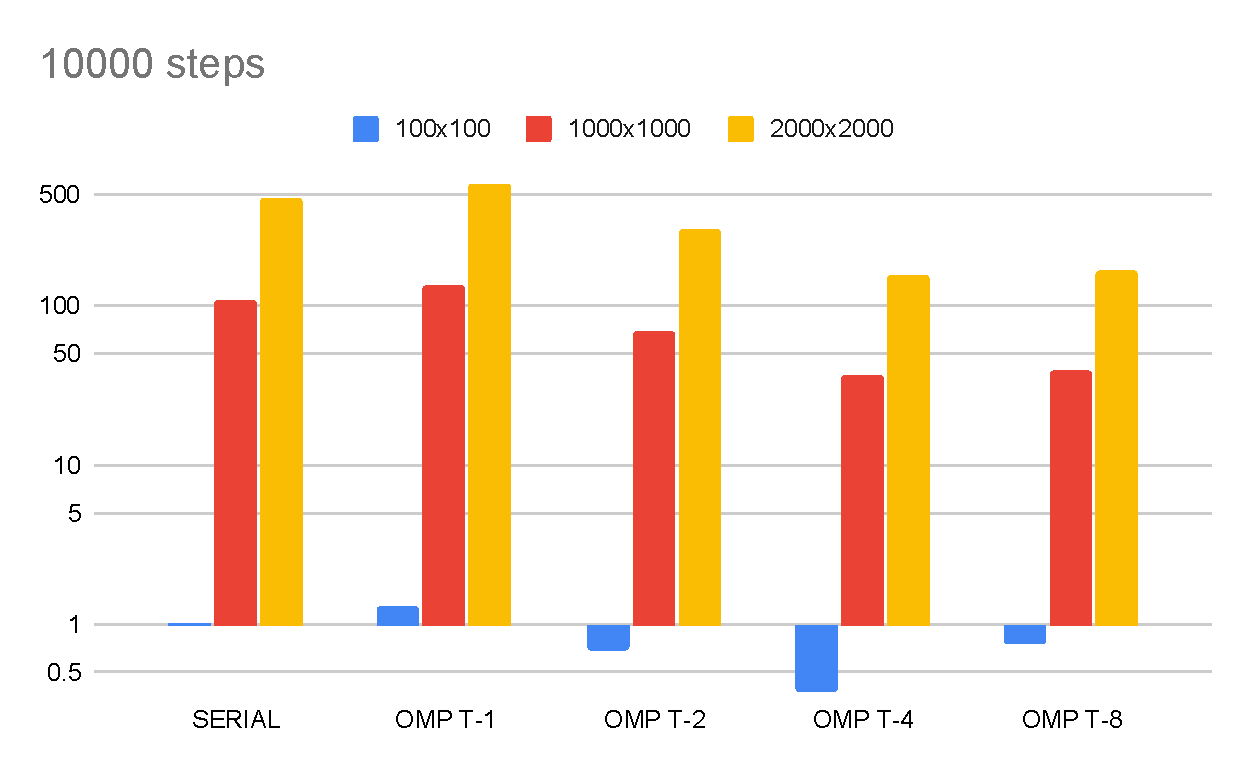
\includegraphics[width=0.9\linewidth]{\subfix{../media/figures/10000 steps.pdf}}
        \caption{Execution time comparison between different matrix sizes}
        \label{fig:10000-steps}
    \end{subfigure}
    \begin{subfigure}{0.7\textwidth}
        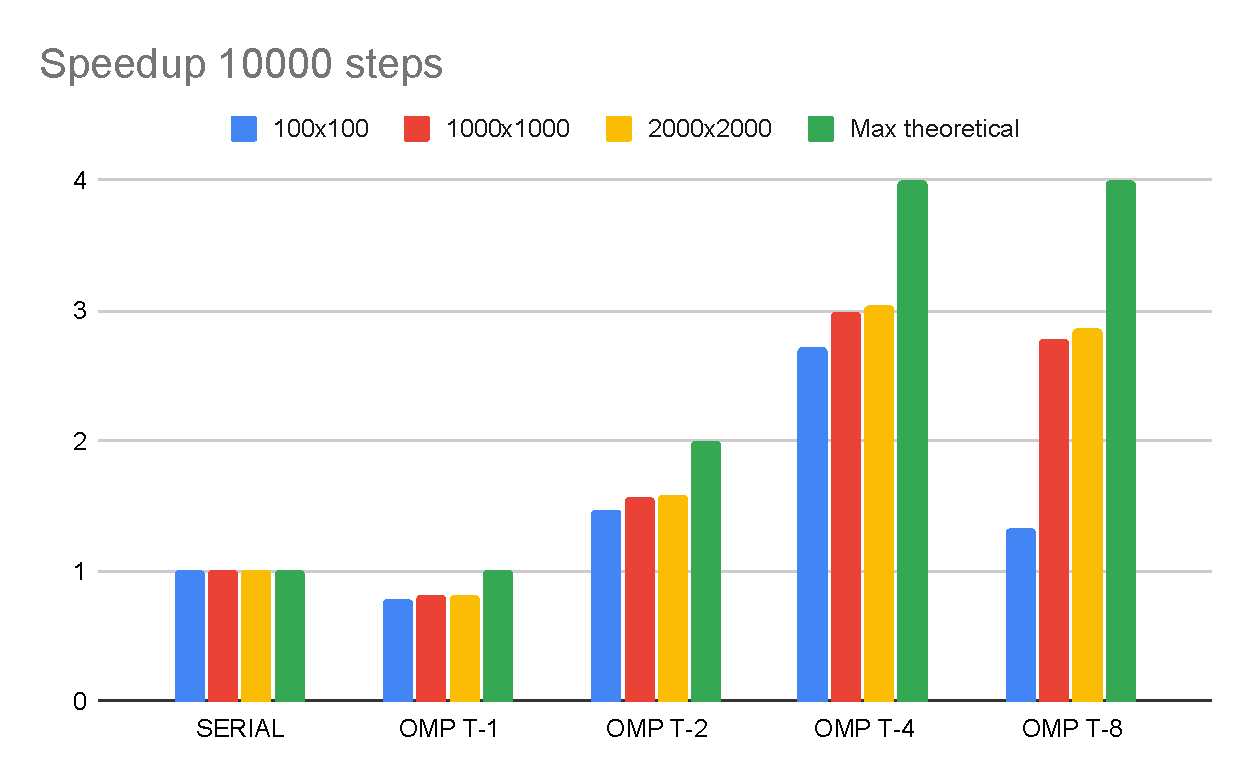
\includegraphics[width=0.9\linewidth]{\subfix{../media/figures/Speedup 10000 steps.pdf}}
        \caption{Speedup comparison of the different executions}
        \label{fig:10000-steps-speedup}
    \end{subfigure}
    \begin{subfigure}{0.7\textwidth}
        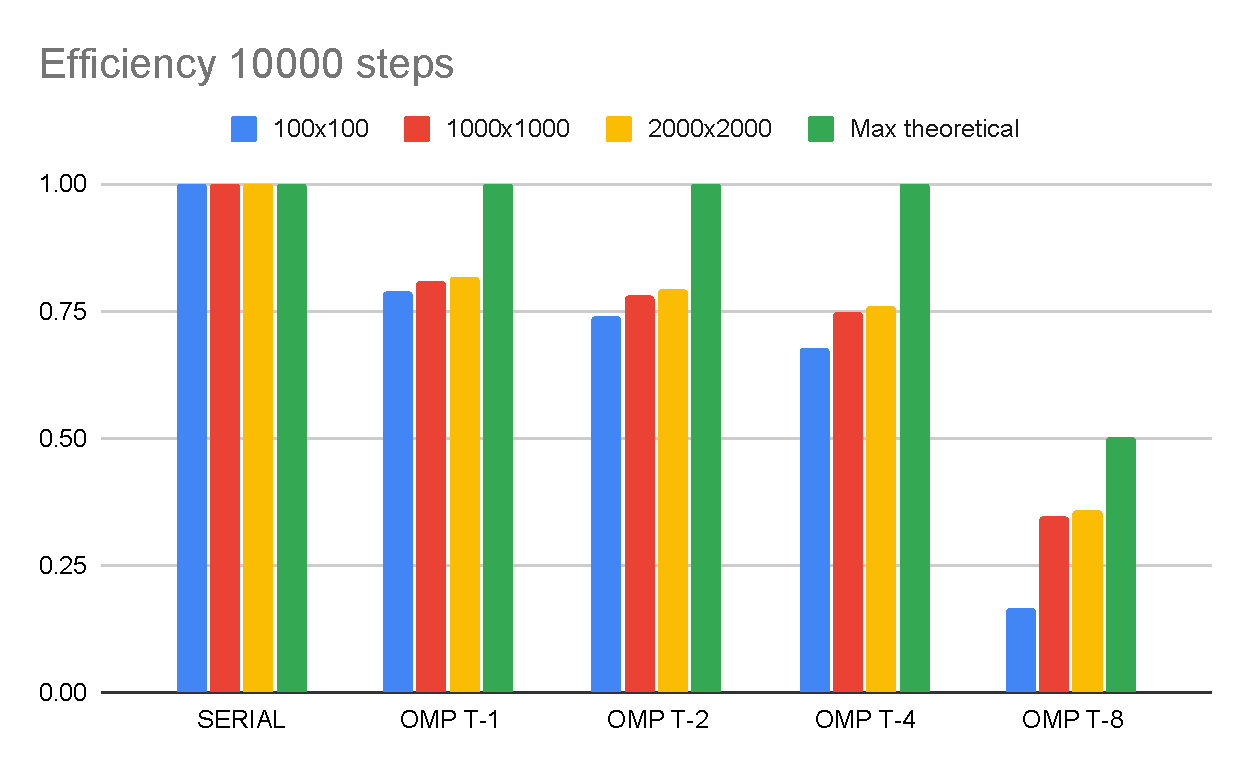
\includegraphics[width=0.9\linewidth]{\subfix{../media/figures/Efficiency 10000 steps.pdf}}
        \caption{Efficiency comparison of the different executions}
        \label{fig:10000-steps-efficiency}
    \end{subfigure}
    \caption{Time, speedup and efficiency graphs of \textit{10000 steps} execution}
\end{figure}

\subsection{\textit{100000 steps} results}

Executions using \textit{100000 steps}, \textit{Figure \ref{fig:100000-steps}}, \textit{Figure \ref{fig:100000-steps-speedup}} and \textit{Figure \ref{fig:100000-steps-efficiency}}. 


\begin{figure}[!htb]
    \centering
    \label{fig:100000-steps-all}
    \begin{subfigure}{0.7\textwidth}
        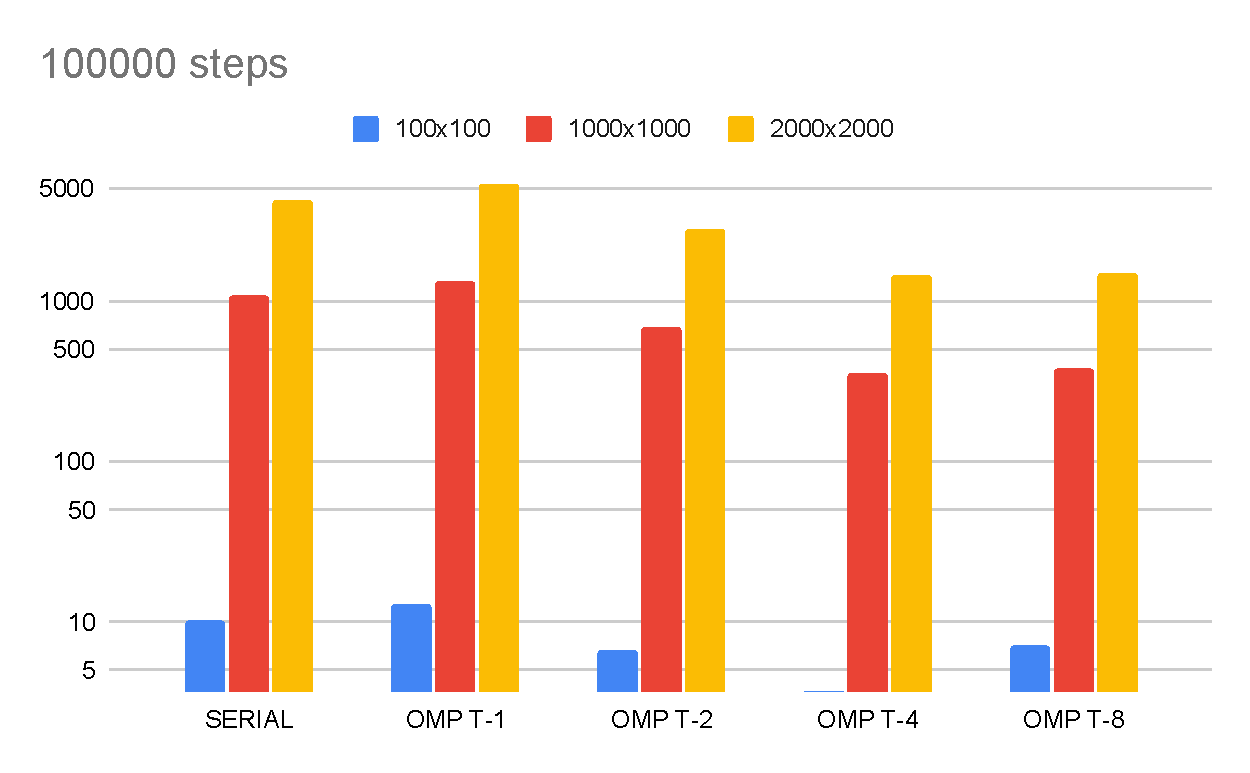
\includegraphics[width=0.9\linewidth]{\subfix{../media/figures/100000 steps.pdf}}
        \caption{Execution time comparison between different matrix sizes}
        \label{fig:100000-steps}
    \end{subfigure}
    \begin{subfigure}{0.7\textwidth}
        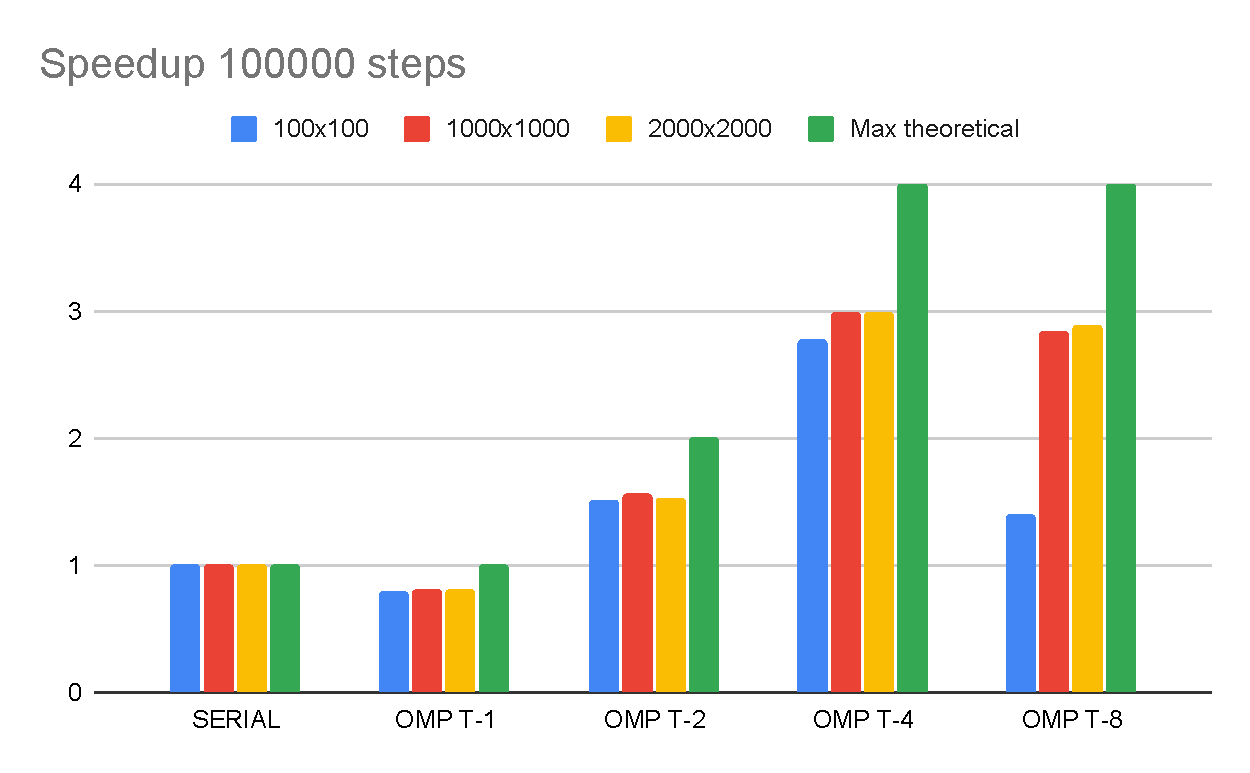
\includegraphics[width=0.9\linewidth]{\subfix{../media/figures/Speedup 100000 steps.pdf}}
        \caption{Speedup comparison of the different executions}
        \label{fig:100000-steps-speedup}
    \end{subfigure}
    \begin{subfigure}{0.7\textwidth}
        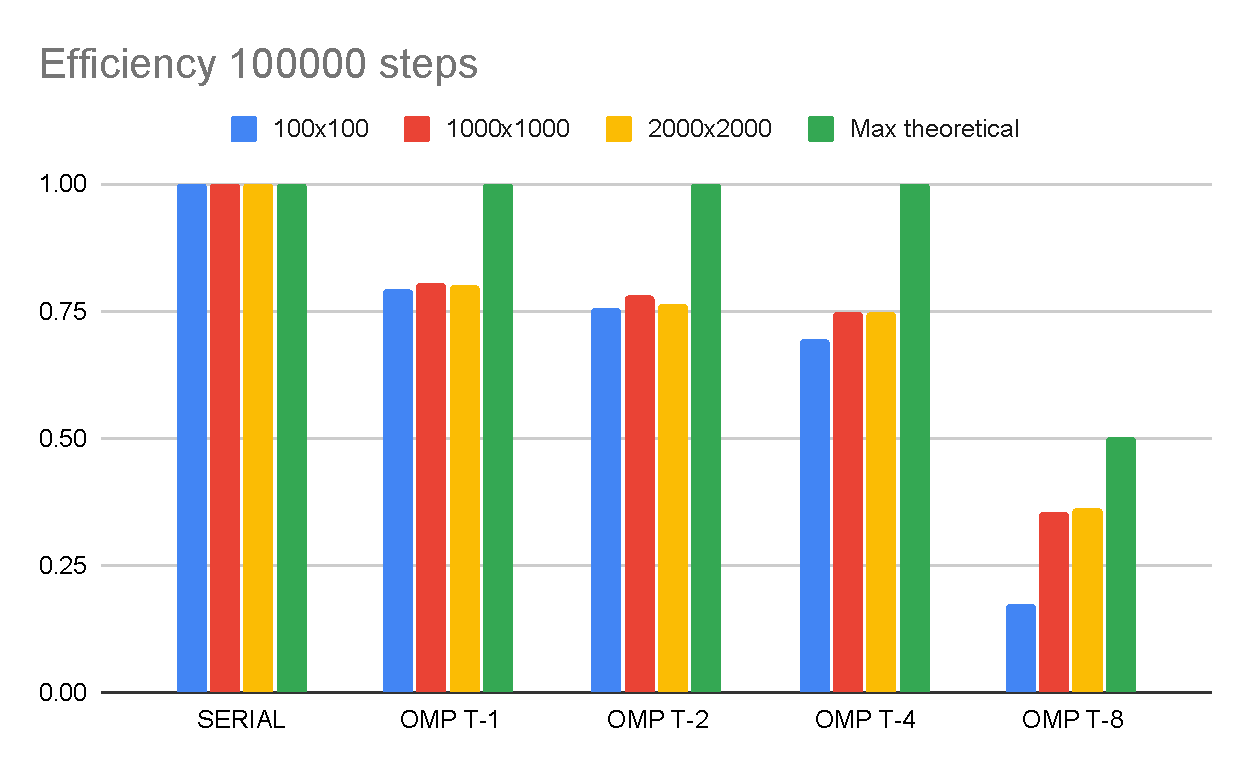
\includegraphics[width=0.9\linewidth]{\subfix{../media/figures/Efficiency 100000 steps.pdf}}
        \caption{Efficiency comparison of the different executions}
        \label{fig:100000-steps-efficiency}
    \end{subfigure}
    \caption{Time, speedup and efficiency graphs of \textit{100000 steps} execution}
\end{figure}


\end{document}